\section{Repetitionsopgaver}
\begin{enumerate}
	\item Udregn følgende
	\begin{align*}
	\frac{2}{3}-\frac{3}{4},&& \frac{\frac{4}{6}+\frac{1}{3}}{2},&& \frac{\frac{2}{3}}{\frac{1}{5}} \cdot \frac{2}{5}+\frac{1}{2}.
	\end{align*}
	\item Løs ligningerne
	\begin{align*}
	\frac{x}{5}+2=7,&& 2x^2-3x=2,&& \frac{3}{x}=x+2,&& x^4-6x^2+8=0.
	\end{align*}
	\item Reducer følgende
	\begin{align*}
	\frac{x^2+4-4x}{x^2+x-6},&& \frac{9-x^2}{x^2-2x-3}.
	\end{align*}
	\item Udregn følgende
	\begin{align*}
	(3x^2)^3,&& \frac{x^2y}{(xy)^2},&& \frac{x^2}{\sqrt{x}^3}.
	\end{align*}
	\item Løs ligningssystemet 
	\begin{alignat*}{3}
	4y&{}+{}&3x&{}={}&4\\
	2y&{}-{}&x&{}={}&-3
	\end{alignat*}
	\item Afgør om funktionerne $f$ og $g$ afbildet i Figur~\ref{fig:funktioner1et} og Figur~\ref{fig:funktioner1to} er surjektive, injektive og/eller bijektive.
	\begin{figure}[!htbp]
		\begin{minipage}{0.49\textwidth}
			\pgfplotsset{width=0.5\textwidth,compat=1.11}
			\centering
			\begin{tikzpicture}
			\draw \boundellipse{0,0}{0.7}{1.4};
			\draw \boundellipse{3,0}{0.7}{1.4};
			\node[circle,fill,inner sep=1pt] at (0.05,1.0) [label=left:$a$]{};
			\node[circle,fill,inner sep=1pt] at (0.05,0.35) [label=left:$b$]{};
			\node[circle,fill,inner sep=1pt] at (0.05,-0.35) [label=left:$c$]{};
			\node[circle,fill,inner sep=1pt] at (0.05,-1.0) [label=left:$d$]{}; 
			\node[] at (0.45,1.7) [label=left:$X$]{}; 
			\node[circle,fill,inner sep=1pt] at (3.0,0.7) [label=right:1]{};
			\node[circle,fill,inner sep=1pt] at (3.0,0.0) [label=right:2]{};
			\node[circle,fill,inner sep=1pt] at (3.0,-0.7) [label=right:3]{}; 
			\node[] at (3.45,1.7) [label=left:$Y$]{}; 
			\node[] at (1.9,1.3) [label=left:$g$]{}; 
			\draw[->,thick] (0.2,1.0) -- (2.8,0.07);
			\draw[->,thick] (0.2,0.35) -- (2.8,0.7);
			\draw[->,thick] (0.2,-0.35) -- (2.8,-0.07);
			\draw[->,thick] (0.2,-1.0) -- (2.8,-0.7);
			\end{tikzpicture}
			\caption{$g$}
			\label{fig:funktioner1et}
		\end{minipage}
		\begin{minipage}{0.49\textwidth}
			\centering
			\pgfplotsset{width=0.5\textwidth,compat=1.11}
			\centering
			\begin{tikzpicture}
			\draw \boundellipse{0,0}{0.7}{1.4};
			\draw \boundellipse{3,0}{0.7}{1.4};
			\node[circle,fill,inner sep=1pt] at (0.05,0.7) [label=left:$a$]{};
			\node[circle,fill,inner sep=1pt] at (0.05,0.0) [label=left:$b$]{};
			\node[circle,fill,inner sep=1pt] at (0.05,-0.7) [label=left:$c$]{}; 
			\node[] at (0.45,1.7) [label=left:$X$]{}; 
			\node[circle,fill,inner sep=1pt] at (3.0,1.0) [label=right:1]{};
			\node[circle,fill,inner sep=1pt] at (3.0,0.35) [label=right:2]{};
			\node[circle,fill,inner sep=1pt] at (3.0,-0.35) [label=right:3]{};
			\node[circle,fill,inner sep=1pt] at (3.0,-1.0) [label=right:4]{}; 
			\node[] at (3.45,1.7) [label=left:$Y$]{}; 
			\node[] at (1.9,1.3) [label=left:$f$]{}; 
			\draw[->,thick] (0.2,0.7) -- (2.8,1);
			\draw[->,thick] (0.2,0.0) -- (2.8,0.40);
			\draw[->,thick] (0.2,-0.7) -- (2.8,0.30);
			\end{tikzpicture}
			\caption{$f$}
			\label{fig:funktioner1to}
		\end{minipage}
	\end{figure}
	
	\item Funktionerne $f$, $g$ og $h$ opfylder $f(3)=-1$, $g(-1)=2$ og $h(2)=-1$. Bestem $h(g(-1))$ og $ g(f(3)) $.
	
	\item Lad $f(x)=\frac{1}{1+x^2}$ og $g(x)=\cos^2(x)$. Bestem $f(g(x))$ og $g(f(x))$.
	
	\item Udregn følgende:
	\begin{align*}
	\ln((e^{3})^2),&& 8^{\log_2(3)},&& e^{\frac{1}{\ln(e^{-3})}}.
	\end{align*}
	
	\item Løs ligningerne
	\begin{align*}
	e^{x^2+1}=e^{2x}, && \ln(2x+1)+\ln(x)=0
	\end{align*}
	
	\item Udregn følgende:
	\begin{align*}
	\cos(\frac{\pi}{2}+\frac{\pi}{3})\tan(\frac{2\pi}{3}),&&\frac{\sin(\frac{2\pi}{3})-\cos(\frac{\pi}{4}-\frac{13\pi}{12})}{\tan(\frac{\pi}{6})}.
	\end{align*}
	
	\item Bestem alle punkter hvor funktionen $f$ givet ved
	\begin{align*}
	f(x)=\begin{cases}
	0,& \textup{når } x<0\\
	1,& \textup{når } 0\leq x<1\\
	2,&\textup{når } 1\leq x<2\\
	3,&\textup{ellers}
	\end{cases}
	\end{align*}
	er kontinuert.
	
	\item Bestem $\lim_{x\to 2} xe^{x^2-4}-x$.
	
	\item Differentier funktionerne
	\begin{align*}
	f(x)=2x^2-\frac{1}{\sqrt{x}},&&g(x)=\sqrt[3]{x^2}-\cos(x),&& h(x)=\ln(x^{\frac{3}{2}})+(e^{2x})^{x}.
	\end{align*}
	
	\item Differentier funktionerne
	\begin{align*}
	f(x)=\tan(x^2),&& g(x)=e^{2\sin(x)}\sin(x),&& h(x)=xe^{-3\ln(\sqrt{x})}
	\end{align*}
	
	
	\item\label{it:rep1} Bestem for hver af de blå grafer i Figur~\ref{fig:rep1} hvilken af de røde grafer
	der beskriver den afledede.
	\begin{figure}
		\centering
		
		\begin{minipage}{0.3\linewidth}
			\begin{tikzpicture}[scale=0.5]
			\begin{axis}[xmin=-2,xmax=2,ymin=-2,ymax=2,axis x line=center,
			axis y line=center,ticks=none]
			\addplot[thick,blue, samples = 600] {e^(-x^2)};
			\end{axis}
			\end{tikzpicture}
		\end{minipage}
		\begin{minipage}{0.3\linewidth}
			\begin{tikzpicture}[scale=0.5]
			\begin{axis}[xmin=-2,xmax=2,ymin=-2,ymax=2,axis x line=center,
			axis y line=center,ticks=none,restrict y to domain=-2:2]
			\addplot[thick,blue, samples = 700]  {sin(deg(x))*(x^2)^(1/3)};
			\end{axis}
			\end{tikzpicture}
		\end{minipage}
		\begin{minipage}{0.3\linewidth}
			\begin{tikzpicture}[scale=0.5]
			\begin{axis}[xmin=-2,xmax=2,ymin=-2,ymax=2,axis x line=center,
			axis y line=center,ticks=none, restrict y to domain=-2:2]
			\addplot[thick,blue, samples = 600] {-ln(cos(deg(sin(2*deg(x))^2)))};
			\end{axis}
			\end{tikzpicture}
		\end{minipage}
		
		\begin{minipage}{0.3\linewidth}
			\begin{tikzpicture}[scale=0.5]
			\begin{axis}[xmin=-2,xmax=2,ymin=-2,ymax=2,axis x line=center,
			axis y line=center,ticks=none]
			\addplot[thick,red, samples = 600] {-2*x*e^(-x^2)};<
			\end{axis}
			\end{tikzpicture}
		\end{minipage}
		\begin{minipage}{0.3\linewidth}
			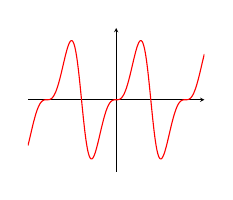
\begin{tikzpicture}[scale=0.5]
			\begin{axis}[xmin=-2,xmax=2,ymin=-2,ymax=2,axis x line=center,
			axis y line=center,ticks=none]
			\addplot[domain=-2:2,thick,red, samples = 600] {4*sin(2*deg(x))*cos(2*deg(x))*tan(deg(sin(2*deg(x))^2))};
			\end{axis}
			\end{tikzpicture}
		\end{minipage}
		\begin{minipage}{0.3\linewidth}
			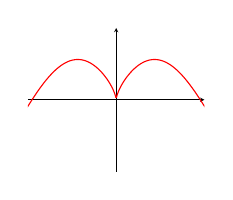
\begin{tikzpicture}[scale=0.5]
			\begin{axis}[xmin=-2,xmax=2,ymin=-2,ymax=2,axis x line=center,
			axis y line=center,ticks=none]
			\addplot[thick,red, samples = 600] {x*(2*sin(deg(x))+3*x*cos(deg(x)))/(3*((x^2)^2)^(1/3))};					
			\end{axis}
			\end{tikzpicture}
		\end{minipage}
		\caption{Opgave~\ref{it:rep1}}
		\label{fig:rep1}
	\end{figure}	
	
	\item Lad funktionen $f$ være givet ved $f(x)=x^2+\cos(x)-4$ og lad $g$ være en funktion som opfylder at $g(3)=\frac{\pi}{6}$ og at $g'(3)=-\frac{1}{2}$. Bestem $(f\circ g)'(3)$. 
	
	
	\item Bestem monitoniforholdene for funktionen $f(x)=x^2+4-4x$ og find tangentligningen gennem punktet $(1,f(1))$.
	
	\item Bestem ekstremumsværdierne for $f(x)=3x^2+2x+4$ i intervallet $[-1,1]$.
	
	\item I \href{https://www.geogebra.org/m/jz34tfh5}{Geogebra} er en ligesidet trekant med sidelængder 1 skitseret i et koordinatsystem. I trekanten er tegnet et indskrevet rektangel som er symmetrisk om linjen $x=\frac{1}{2}$. Bestem det størst mulige areal af rektanglet. 
	
	\item Er $F(x)=12\sqrt{x}-2x^2+1$ en stamfunktion til $f(x)=\frac{6}{\sqrt{x}}+4x$?
	

	\item Udregn følgende integraler
	\begin{align*}
	\int x^2+1\dd x,&& \int \frac{x}{\sqrt{x}}+\sin(x)\dd x,&& \int \frac{1}{2}e^{\frac{x}{2}}\dd x.
	\end{align*}

		\item Udregn følgende integraler
	\begin{align*}
	\int x\cos(x)\dd x,&& \int x^2 \ln(x)\dd x.
	\end{align*}
	
	\item Udregn følgende integraler
	\begin{align*}
	3\int (x^2+1)e^{x^3+3x-1}\dd x,&& \int x\ln(x^2) \dd x, && \int \frac{4x^3+2x-1}{e^{x^4+x^2-x}} \dd x.
	\end{align*}
	
	\item Udregn følgende bestemte integraler
	\begin{align*}
	2\int_0^1 x^2+1\dd x,&& \int_{-3}^{3} x^3-3x\dd x,&& \int_{-1}^0 xe^x \dd x.
	\end{align*}
	
	\item Udregn følgende bestemte integraler:
	\begin{align*}
	\int_{-1}^0 2xe^{x^2}\dd x,&& \int_{0}^{-\sqrt{\pi}} 5x\cos(x^2)\dd x.
	\end{align*}
	
	\item\label{it:rep2} Lad $f\colon [0,2\pi]\to \R$ være givet ved
	\begin{align*}
	f(x)=\begin{cases}
	\cos(x)-\sin(x),&\textup{hvis } 0\leq x<\frac{\pi}{4}\\
	\sin(x)-\cos(x),& \textup{hvis } \frac{\pi}{4}\leq 0<\frac{5\pi}{4}\\
	\cos(x)- \sin(x),&\textup{hvis } \frac{5\pi}{4}\leq x\leq 2\pi.
	\end{cases}
	\end{align*} 
	Grafen for $f$ er plottet i Figur~\ref{fig:rep2}. Bestem arealet mellem $x$-aksen og $f$ i intervallet $[0,2\pi]$.
		\begin{figure}
		\centering
		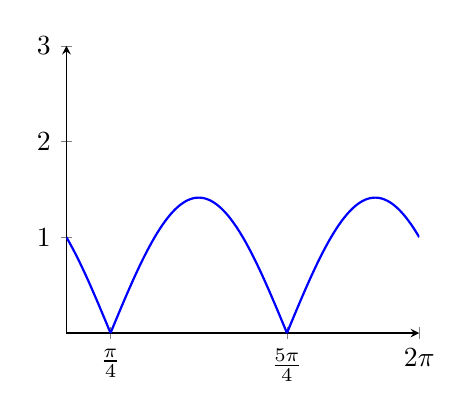
\begin{tikzpicture}
		\begin{axis}[xmin=0,xmax=2*pi,ymin=0,ymax=3,axis x line=center,
		axis y line=center,xtick={0,pi/4,5*pi/4,2*pi},xticklabels={0,$\frac{\pi}{4}$,$ \frac{5\pi}{4} $,$ 2\pi $}]
		\addplot[blue,thick,samples=200,domain=0:pi/4] {cos(deg(x))-sin(deg(x))};
		\addplot[blue,thick,samples=200,domain=pi/4:5*pi/4] {-(cos(deg(x))-sin(deg(x)))};
		\addplot[blue,thick,samples=200,domain=5*pi/4:2*pi] {cos(deg(x))-sin(deg(x))};
		\end{axis}
		\end{tikzpicture}
		\caption{Opgave~\ref{it:rep2}}
		\label{fig:rep2}
	\end{figure}
	
	\item Bestem en løsning til differentialligningen
	\begin{align*}
	y'+3y=0.
	\end{align*}
	
	\item Vis at $ f(x)=e^{-e^x} $ er en løsning til differentialligningen
	\begin{align*}
	-\frac{y'}{y}=e^x
	\end{align*}
	
	\item Hvilke af funktionerne
	\begin{align*}
	y_1(x)=\cos(3x),&&y_2(x)=3\sin(3x),&& y_3(x)=2e^{-3x},&& y_4(x)=3x^3
	\end{align*}
	løser differentialligningen
	\begin{align*}
	-y''=9y?
	\end{align*}
	
	\item Differentialligningen 
	\begin{align*}
	y'-y=x
	\end{align*}
	har en løsning som går gennem punktet $(-\ln(2),\ln(2))$. Bestem ligningen for tangenten til løsningen i dette punkt.
	
	\item Vis at $y_1(x)=\cos x$ og $y_2(x)=\sin x$ er løsninger til differentialligningssystemet
	\begin{align*}
	y_1'&=-y_2\\
	y_2'&=y_1,
	\end{align*}
	med begyndelsesværdibetingelserne $y_1(0)=1$ og $y_2(0)=0$. 
	
	\item Bestem den fuldstændige løsning til differentialligningen
	\begin{align*}
	y'+xy=x.
	\end{align*}
	
	\item Bestem den fuldstændige løsning til differentialligningen
	\begin{align*}
	y'-\sin(x)y=\sin(x).
	\end{align*}
	
	\item Hvilke af funktionerne
	\begin{align*}
	y_1(x)=\frac{-1}{4}\cos(2x),&& y_2(x)=\frac{1}{4}\sin(2x)&& y_3(x)=\frac{-1}{2}\cos^2(x),&& y_4(x)=\frac{1}{2}\sin^2(x)
	\end{align*}
	 løser differentialligningen
	\begin{align*}
	y'=\sin(x)\cos(x)?
	\end{align*}
	
	\item Lad 
	\begin{align*}
	\vec{u}=\begin{bmatrix}
	4\\-2
	\end{bmatrix},\quad \textup{og}\quad \vec{v}=\begin{bmatrix}
	-1\\-2
	\end{bmatrix}.
	\end{align*}
	Udregn
	\begin{align*}
	-\vec{u},&&2\vec{v},&&\vec{u}+\vec{v},&&\vec{u}-3\vec{v},&&\norm{\vec{u}},&&\norm{\vec{v}},&&\vec{u}\c \vec{v},&& \hat{\vec{u}}\c (3\vec{v}).
	\end{align*}
	
		\item Bestem arealet af det parallelogram som udspændes af de to vektorer
	\begin{align*}
	\vec{u}=\begin{bmatrix}
	1\\3
	\end{bmatrix},
	\vec{v}=\begin{bmatrix}
	1\\-2
	\end{bmatrix}.
	\end{align*}
	
		
	\item Vis at vektorerne 
	\begin{align*}
	\vec{u}=\begin{bmatrix}
	\frac{\sqrt{2}}{2}\\\frac{-\sqrt{2}}{2}
	\end{bmatrix},
	\vec{v}=\begin{bmatrix}
	\frac{-\sqrt{2}}{2}\\\frac{-\sqrt{2}}{2}
	\end{bmatrix}
	\end{align*}
	er ortogonale og begge har norm 1.
	
	\item Linjen $l$ har ligning 
	\begin{align*}
	3x+-2y=1
	\end{align*}
	og linjen $m$ har parameterfremstilling
	\begin{align*}
	\begin{bmatrix}
	x\\y
	\end{bmatrix}= \begin{bmatrix}
	-1\\1
	\end{bmatrix}+t \begin{bmatrix}
	-1\\-1
	\end{bmatrix}
	\end{align*}
	hvor $t\in \R$. Er $l$ og $m$ er parallelle?
	
	
	\item  Lad 
	\begin{align*}
	\vec{u}=\begin{bmatrix}
	1\\-1\\2
	\end{bmatrix},\quad \textup{og}\quad \vec{v}=\begin{bmatrix}
	0\\1\\-3.
	\end{bmatrix}.
	\end{align*}
	Udregn
	\begin{align*}
	-\vec{u},&&-2\vec{v},&&\vec{u}+\vec{v},&&\vec{u}-\vec{v},&&\norm{\vec{u}},&&\norm{\vec{v}},&&\vec{u}\c \vec{v},&& \vec{u}\times \vec{v}.
	\end{align*}
	
	\item Bestem arealet af parallelogrammet udspændt af vektorerne
	\begin{align*}
	\vec{u}=\begin{bmatrix}
	3\\-1\\2
	\end{bmatrix},\quad \textup{og}\quad \vec{v}=\begin{bmatrix}
	0\\2\\2.
	\end{bmatrix}.
	\end{align*}
	
	\item Bestem en parameterfremstilling for linjen $m$ gennem punkterne $P_1 =
	(2, 3,-1)$ og $P_2 = (2,-2, 0)$. Ligger $P = (2, 8, -2)$ på $m$?
	
	\item Bestem en ligning for planen der indeholder $P=(1,1,1)$ og har normalvektor
	\begin{align*}
	\vec{u}=\begin{bmatrix}
	2\\-1\\3
	\end{bmatrix}.
	\end{align*}
	Ligger $P_1=(2,-1,\frac{-1}{3})$ i planen?
\end{enumerate}